\documentclass[../main.tex]{subfiles}

\begin{document}


\section{Computation}

Given a set of physicians $\{(V_j, \tau_j, R_j(\cdot),P_j(\cdot))\}_{j =1}^{J}$, the distribution functions for patient parameters $F(\kappa)$ and $G(\gamma)$, and one search model parameter $z$, which is $\lambda$ in the Logit model, $\beta$ in the sequential model, we develop an algorithm to compute market equilibrium.

Equilibrium aggregates are computed on the basis of Monte-Carlo matrix calculus. Set $J$ as the number of physicians\footnote{Or, as we'll later interpret it, as the number of bins, where each bin $j$ is a unique combination of $ (V_j, \tau_j, R_j(\cdot),P_j(\cdot))$.}, $I$ as the size of the sample drawn randomly from $F(\kappa)$ and $G(\gamma)$. For both models we define a class which can output a matrix $S$ where each column is a patient's strategy vector $S_i$ following that model, when given as input the arrayed set of physicians' quality and visit cost $\{(V_j, \tau_j)\}_{i =1}^{J}$, an arrayed set of patients $(\{(\kappa_i,\gamma_i)\}_{i =1}^{I}$, the model parameter $z$ and a given vector of physician strategies $\{\bar{\kappa_j}\}_{j =1}^{J}$.

We input as ``patients'' our $I$ samples from $F(\kappa)$ and $G(\gamma)$, then a $J \times I$ matrix $U$ is computed, where each component $u_{ji}$\footnote{As we have defined our matrices $J \times I$ for ease of visualization, we will refer to matrix components as $x_{ji}$ in this section rather than $x_{ij}$ as we do elsewhere in the paper.} corresponds to the utility the sampled patient $i$ would get from a visit to physician $j$. This step is the same for both classes.

What differs between both models is the computation of the matrix $S$ of patient strategis out of the utility matrix $U$:

\begin{itemize}
    \item \textbf{Implicit search model (Logit):} First, an `$\alpha$-matrix' is calculated over matrix $U,$ where each $\alpha_{ji}$ is $e^{\lambda u_{ji}}$ if $u_{ji} > 0$ and $0$ if not. Then, for each patient $i$, that is, for each column, each component $s_{ji}$ of the $S$ matrix takes on the values $s_{ji} = \alpha_{ji}/\sum_{k = 1}^{J} \alpha_{ki}$.

    \item \textbf{Explicit search model (Sequential):} Recall equation (NUMBER) characterizing patient thresholds. We first compute the $I$-dimensional vector of the sampled patients' respective $\bar{U_i}$. Define $U_i$ as the set $\{u_{ji}\}_{j=1}^{J}$ of utility patient $i$ recieves from a visit to each physician. In matrix terms $U_i$ would be the $i$th column of the $J \times I$ matrix $U$. The operation to compute each $\bar{U_i}$ is the following:
    \begin{equation}
    \bar{U_i} \equiv \argmin_{x \, \in \, U_i}\; \left\|  \; x - \frac{\beta}{1-\beta}  \sum_{j=1}^{J} \left\{ \frac{\mathbbm{1}[ u_{ji} \geq x ] \cdot (u_{ji} - x)}{\mathbbm{1}[ u_{ji} \geq x ]} \right\} \right\|
    \label{eq:comp1}
    \end{equation}
    where the norm $\| \cdot \|$ is defined in $\mathbb{R}$ as simply the absolute value $| \cdot |$. This is to say, for each sampled patient $i$ we evaluate $x$ for each $u_{ji}$ in $U_i$. In plain words, if patient $i$ where to say: ``I will only visit physicians which grant me at least as much utility as physician $j$'', the optimal choice of $j$ and its respective $u_{ji}$ would be the minimal in $U_i$ for the evaluation of the absolute value in the left-hand side of (\ref{eq:comp1}). This is computationally less intensive than seeking to compute the exact root of (NUMBER), which would be a redundant exercise, because there's a discrete number of physicians above that mark, and selecting instead to use ``the lowest $u_{ji}$ above the root of (NUMBER)'' as threshold instead of the root proper would result in the same vector of strategies $S_i$ for each patient.\footnote{Granted, this is not strictly true, as in our formulation a `$u_{ji}$' may be selected as threshold which is actually below the root proper in $\mathbb{R}$, but closer to it than the nearest one above it. The effect of this ``estimation noise'' on our overall results is negligible.}

    Once having computed our $I$-dimensional vector of patients' $\bar{U_i}$, we evaluate column-wise the binary operator $\mathbbm{1}\{u_{ji}\geq \bar{U_i}\}$ over matrix $U$, and the $J \times I$ matrix $S$ of patient strategies takes on the values $s_{ji} = \mathbbm{1}\{u_{ji}\geq \bar{U_i}\} / \sum_{k=1}^{J} \mathbbm{1}\{u_{ki}\geq \bar{U_i}\}$.
\end{itemize}




\newpage

\begin{figure}[H]
    \centering
    \includegraphics[width=0.6\linewidth]{decimals.pdf}
    \vspace{-0.25cm}
\caption{Coefficient $\beta_t$ of \textit{log\_trade} over \textit{log\_distance} over the years, including FEs}
\end{figure}

\begin{figure}[H]
    \centering
    % First subfigure
    \begin{subfigure}[b]{0.45\linewidth}
        \centering
        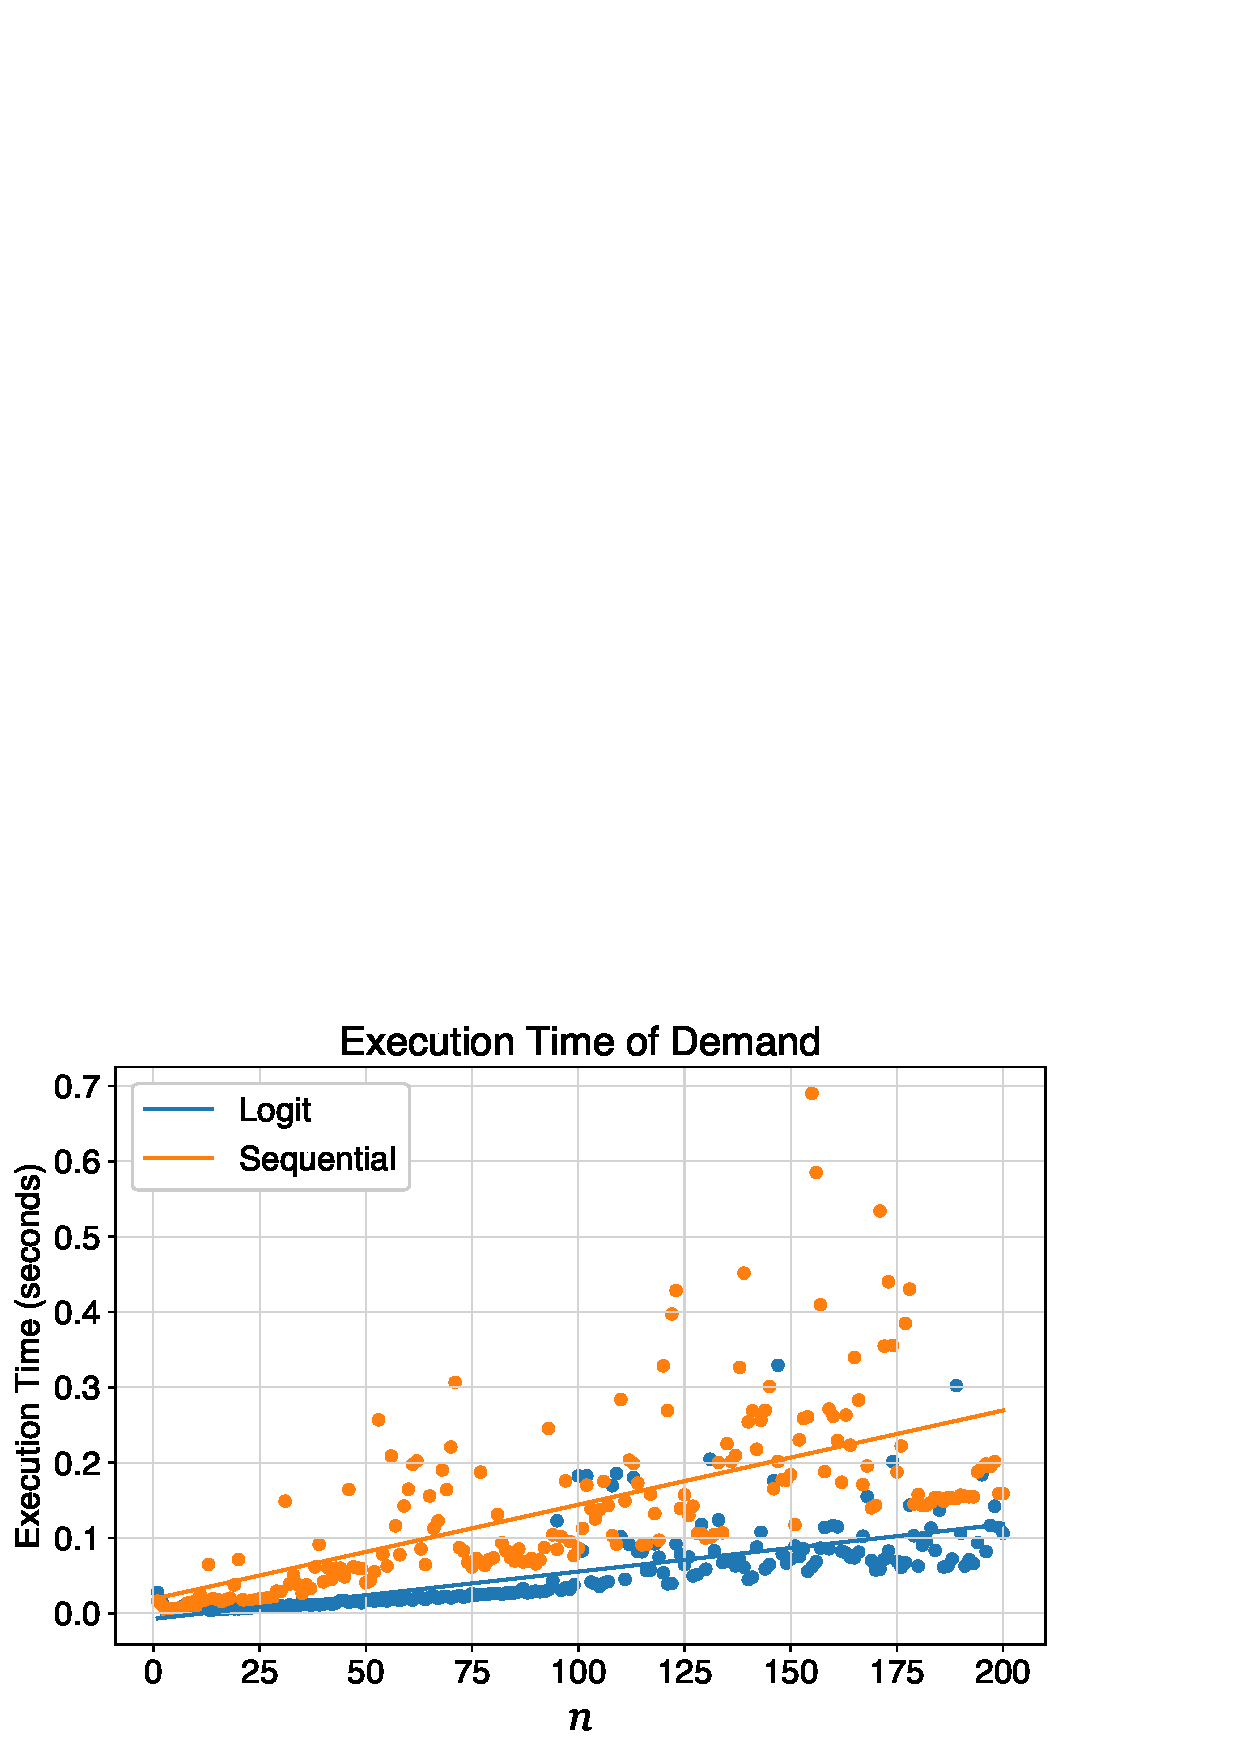
\includegraphics[width=\linewidth]{linear.pdf}
        \vspace{-0.25cm}
        \caption{Coefficient $\beta_t$ of \textit{log\_trade} over} \textit{ for first case}
        \label{fig:subfig1}
    \end{subfigure}
    \hspace{0.05\linewidth}  % Space between the subfigures
    % Second subfigure
    \begin{subfigure}[b]{0.45\linewidth}
        \centering
        \includegraphics[width=\linewidth]{squared.pdf}
        \vspace{-0.25cm}
        \caption{Coefficient $\beta_t$ of \textit{log\_trade} over} \textit{ for second case}
        \label{fig:subfig2}
    \end{subfigure}
    \caption{Comparison of Coefficient $\beta_t$ of \textit{log\_trade} over \textit{log\_distance} over the years, including FEs}
    \label{fig:main_figure}
\end{figure}




\end{document}